
       
\section{Programação por Restrições}

\begin{frame}[fragile]
%[fragile, allowframebreaks=0.9]

    \frametitle{Programação por Restrições (PR) -- I}

   \begin{block}{}
     \begin{itemize}
     
      \item A Programação por Restrições (PR) é conhecida por \textit{Constraint Programming} ou simplesmente \textbf{CP}

      \pause
      \item Uma poderosa teoria (e técnica)  que  contorna a complexidade de certos problemas
      exponenciais
      
       
      \pause
      \item A PR encontrava-se inicialmente dentro da IA e PO, mas como várias outras, tornaram-se
      fortes e autônomas. Atualmente uma área de pesquisa bem forte em alguns países.
      
     
    \end{itemize}
    
    \end{block}
    
\end{frame}




\begin{frame}[fragile]
%[fragile, allowframebreaks=0.9]

    \frametitle{Programação por Restrições (PR) -- II}

   \begin{block}{}
     \begin{itemize}

      \item Aproximadamente o algoritmo da PR é dado:
       \pause       
          \begin{enumerate}

            \item Avaliar algebricamente  os domínios das variáveis com suas restrições

            \item Intercala iterativamente a \textsf{propagação de restrições} com 
                  um \textsf{algoritmo de busca}

            \item A cada variável instanciada, o processo é repetido sobre as demais variáveis, reduzindo progressivamente o espaço de busca

            \item Volte ao passo inicial até que os domínios permaneçam estáticos
            e que as variáveis apresentem instâncias consistentes
              
          \end{enumerate}
       
        \pause
       \item Este núcleo é uma busca por constantes otimizações

        \pause
       \item Uma das virtudes da PR: a legibilidade e clareza de suas soluções
       
    \end{itemize}
    
    \end{block}
    
\end{frame}


\begin{frame}[fragile]
%[fragile, allowframebreaks=0.9]
\frametitle{Programação por Restrições (PR) -- III}

   \begin{block}{}
     \begin{itemize}
    \item Problemas combinatoriais com domínio nos inteiros são bons candidatos a serem
       resolvidos por PR
       \pause
       \item Quando temos problemas que precisamos conhecer \textbf{todas} as respostas, 
    não apenas a melhor resposta
    
      \pause
      \item Quando necessitamos de respostas \textit{precisas} e não apenas as aproximadas.
       Há um custo  computacional a ser pago aqui!
        
        \pause
        \item



    \end{itemize}
    \end{block}
    
\end{frame}



\begin{frame}[fragile]
%[fragile, allowframebreaks=0.9]

\frametitle{Metodologia da  Construção de Modelos}

\begin{figure}[ht!]
\begin{center}

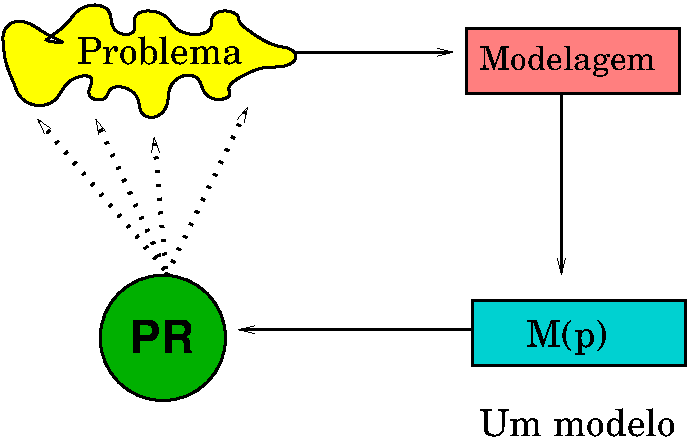
\includegraphics[width=0.70\textwidth, height=0.60\textheight]{figures/problema_modelagem.pdf}

\end{center}
\end{figure}


    
\end{frame}


\begin{frame}[fragile]
%[fragile, allowframebreaks=0.9]

\frametitle{Fluxo de Cálculo da PR}

\begin{figure}[!htb]
\centering
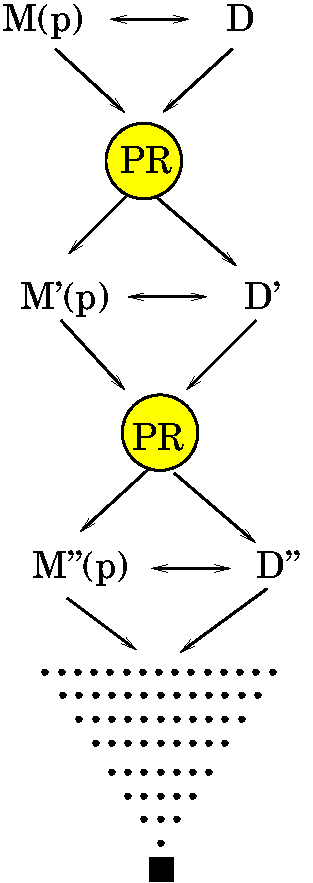
\includegraphics[width=0.30\textwidth, height=0.70\textheight]{figures/dinamica_pr.pdf}
\end{figure}
   
\end{frame}



\begin{frame}[fragile]
%[fragile, allowframebreaks=0.9]

\frametitle{Onde o objetivo da PR é:}

\begin{figure}[!htb]
\begin{center}
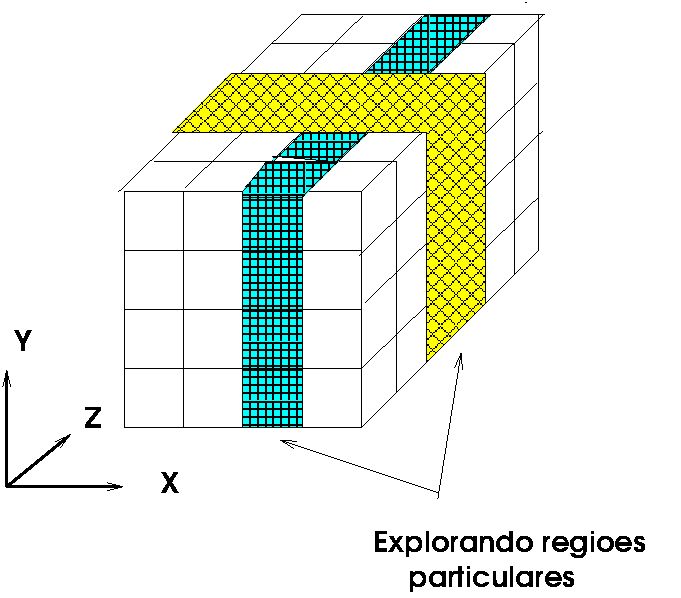
\includegraphics[width=0.70\textwidth, height=0.60\textheight]{figures/reducao_PR_01.pdf}
\caption{Realizar buscas com regiões reduzidas -- promissoras (regiões factíveis de soluções)}
\end{center}
\end{figure}
    
\end{frame}




\begin{frame}[fragile]
%[fragile, allowframebreaks=0.9]

\frametitle{Redução Iterativa em Sub-problemas}

\begin{figure}[!htb]

\begin{center}
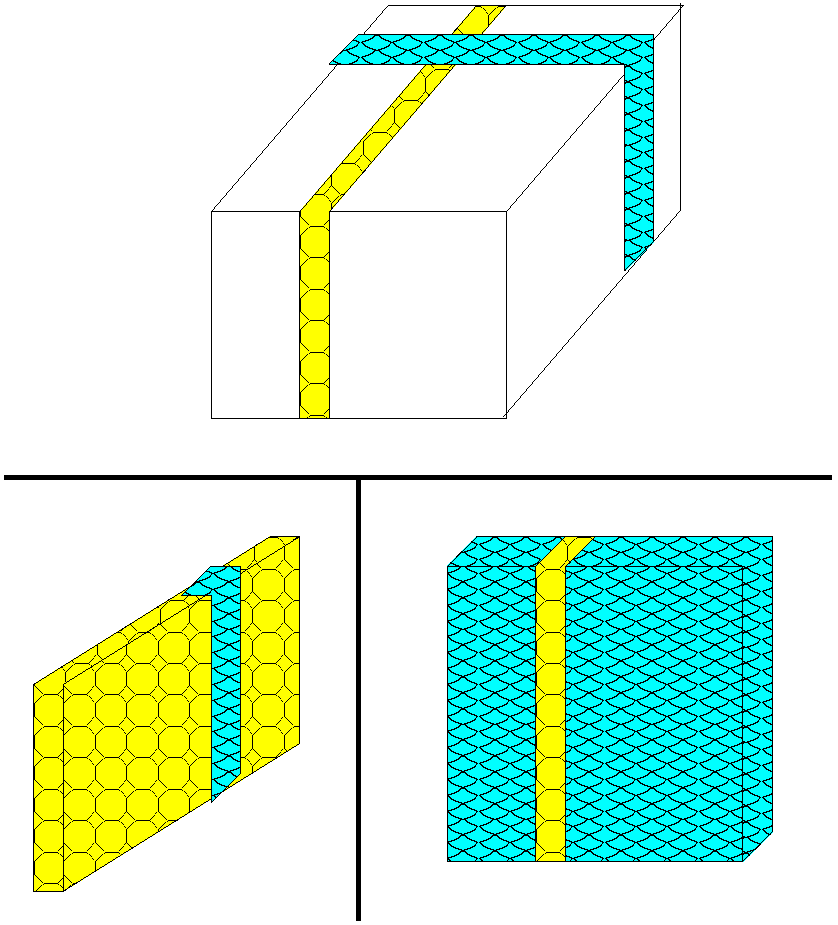
\includegraphics[width=0.70\textwidth, height=0.60\textheight]{figures/reducao_PR_02.pdf}
\caption{Redução de um CP em outros sub-problemas CPs equivalentes}
\end{center}
\end{figure}

    
\end{frame}


\begin{frame}[fragile] 

\frametitle{Exemplo}

\begin{itemize}
  \item Dado um número par qualquer, encontre  dois de números primos, $N_1$ e $N_2$,
diferentes entre si, que somados deêm este número 
par.

\pause
\item Exemplo:\\
Seja o PAR = 18\\
Uma soluç~ao:\\
$N_1 = 7$  e $N_2 = 11$\\
pois\\
$N_1 + N_2 = 18$
\end{itemize}

\end{frame}
\begin{frame}[fragile] 

\frametitle{Modelagem do Problema}

\begin{itemize}
  \item  $N_1$ e $N_2$ assumem valores no domínio dos números primos. \\
  Logo, é importante ter os números primos prontos!

  \pause
   \item A soma destes números é o par fornecido como entrada, $N_{PAR}$:\\
         $N_1 + N_2 = N_{PAR}$

  \pause
  \item  $N_1$ e $N_2$  são diferentes entre si\\
   $N_1 \neq N_2$

  \pause
  \item Como são inteiros: $N_1 < N_{PAR}$ e $N_2 < N_{PAR}$ \\
  Sim, é óbvio, mas isto faz uma redução significativa de domínio!

\end{itemize}

\end{frame}


%%%%%%%%%%%%%%%%%%%%%%%%%%
\begin{frame}[fragile]
 \frametitle{Código Completo}

\begin{itemize}
  \item Acompanhar as explicações do código de:\\
\url{https://github.com/claudiosa/CCS/blob/master/picat/soma_N1_N2_primos_CP.pi}

  \item Confira a execução e testes
\end{itemize}
\end{frame}


%%%%%%%%%%%%%%%%%%%%%%%%%%
\begin{frame}[fragile] 

\frametitle{Código em Partes}

\begin{small}
\begin{verbatim}
modelo => 
    PAR = 382,
    Variaveis = [N1,N2],
    % Gerando um domino soh de primos
    % L_dom = [I : I in 1..1000, eh_primo(I) == true],   %OU
    L_dom = [I : I in 1..1000, prime(I)],
    Variaveis :: L_dom,
\end{verbatim}
\end{small}
   
   Uma ótima estratégia: sair com um domínio de números candidatos!
    
\end{frame}

\begin{frame}[fragile] 

\frametitle{Código em Partes}

\begin{small}
\begin{verbatim}
    % RESTRICOES
    N1 #!= N2,
    N1 #< PAR,  
    N2 #< PAR,
    N1 + N2 #= PAR,
  
	% A BUSCA
	solve([ff], Variaveis),
  % UMA SAIDA
	printf("\n  N1: %d\t N2: %d", N1,N2),
	printf("\n.....................................")
	.
\end{verbatim}
\end{small}
    
\end{frame}

\begin{frame}[fragile] 

\frametitle{Código em Partes}

\begin{small}
\begin{verbatim}
import cp.

% main => modelo	.
% main ?=> modelo, fail.	
% main =>  true.	

main =>
    L = findall(_, $modelo),
    writef("\n Total de solucoes:  %d \n", length(L)) .

\end{verbatim}
\end{small}
    
\end{frame}


\begin{frame}[fragile]
%[fragile, allowframebreaks=0.9]

\frametitle{Saída -- I}

\begin{small}
\begin{verbatim}
Picat> cl('soma_N1_N2_primos_CP').
Compiling:: soma_N1_N2_primos_CP.pi
** Warning  : redefine_preimported_symbol(math): prime / 1
soma_N1_N2_primos_CP.pi compiled in 7 milliseconds
loading...

yes

Picat> main.                      

  N1: 3	 N2: 379
.....................................
  N1: 23	 N2: 359
.....................................
  N1: 29	 N2: 353
.....................................
\end{verbatim}
    
\end{small}
\end{frame}


\begin{frame}[fragile]
%[fragile, allowframebreaks=0.9]

\frametitle{Saída -- II}

\begin{small}
\begin{verbatim}
 .....................................
  N1: 353	 N2: 29
.....................................
  N1: 359	 N2: 23
.....................................
  N1: 379	 N2: 3
.....................................
 Total de solucoes:  18 

yes

Picat> 
\end{verbatim}
    
\end{small}
\end{frame}








\begin{frame}[fragile]
\frametitle{Reflexões}


\begin{itemize}
  \item Há outros métodos para se resolver estes problemas.\\
  Exemplo: Programação Linear, Buscas Heurísticas, etc

  \pause
  \item A área é extensa, contudo, Picat adere há todos requisitos da PR

    \pause
  \item Resumo da PR: segue por uma notação/manipulação algébrica restrita,
  simplificar e bissecionar as restrições, instanciar variáveis, verificar inconsistências,
  avançar sobre as demais variáveis, até que todas estejam instanciadas.
  
\end{itemize}

\end{frame}
